%!TEX root = edance.tex
%%%%%%%%%%%%%%%%
%  CHAPTER 15  %
%%%%%%%%%%%%%%%%
\chapter{Multi-Stage Amplifiers}
\label{ch:ch15_multi_stage_amps}
\graphicspath{{./figures/figs_ch15_multistage/}}
%%%%%%%%%%%%%%%%%%%%%%%%%%%%%%%%%%%%%%%%%%%%%%%%%%%%%%%%%%%%%%%%%%%%%%%%%%%%%%%%%%%%%%%%
%%%%%%%%%%%%%%%%%%%%%%%%%%%%%%%%%%%%%%%%%%%%%%%%%%%%%%%%%%%%%%%%%%%%%%%%%%%%%%%%%%%%%%%%
%                                   SECTION 15.1                                       %
%%%%%%%%%%%%%%%%%%%%%%%%%%%%%%%%%%%%%%%%%%%%%%%%%%%%%%%%%%%%%%%%%%%%%%%%%%%%%%%%%%%%%%%%
%%%%%%%%%%%%%%%%%%%%%%%%%%%%%%%%%%%%%%%%%%%%%%%%%%%%%%%%%%%%%%%%%%%%%%%%%%%%%%%%%%%%%%%%
\section{Chapter Preview}
In this chapter we will be covering multi-stage amplifiers consisting of a \textit{cascade} of two or more single-stage amplifiers.  First we will be reviewing amplifier input/output impedance characteristics, which will provide insights on the best ways to cascade amplifiers.  Next, we will start with the important common source amplifier stage and show that while cascading these stages will result in a higher gain.  However, the higher gain comes with a severe penalty of bandwidth reduction.  To partially circumvent this bandwidth reduction, we will see how voltage buffers can be inserted in between amplifier stages.  We will also cover an important special case of a capacitive load, which commonly occurs for on-chip amplifiers, and how to drive these loads.  The next topology we will investigate in detail is the common source amplifier cascaded with a common gate amplifier, which is better known as the \textit{cascode amplifier}.  We will discuss this topology in detail, because it plays such an important role in circuit design.

The chapter will conclude with a "big" example to demonstrate how a seemingly complex circuit can be simplified into simple building blocks.  Obviously this ability to see through the clutter of a circuit will not be learned overnight, but it is something you can learn fairly quickly through practice.  In many ways we will only touch on the important concepts of multi-stage amplifiers, as the examples in this chapter are fairly simple.  But we must first learn to walk before we attempt to run.
%%%%%%%%%%%%%%%%%%%%%%%%%%%%%%%%%%%%%%%%%%%%
%                 FIGURE                   %
%%%%%%%%%%%%%%%%%%%%%%%%%%%%%%%%%%%%%%%%%%%%
\begin{figure}[H]
\centering
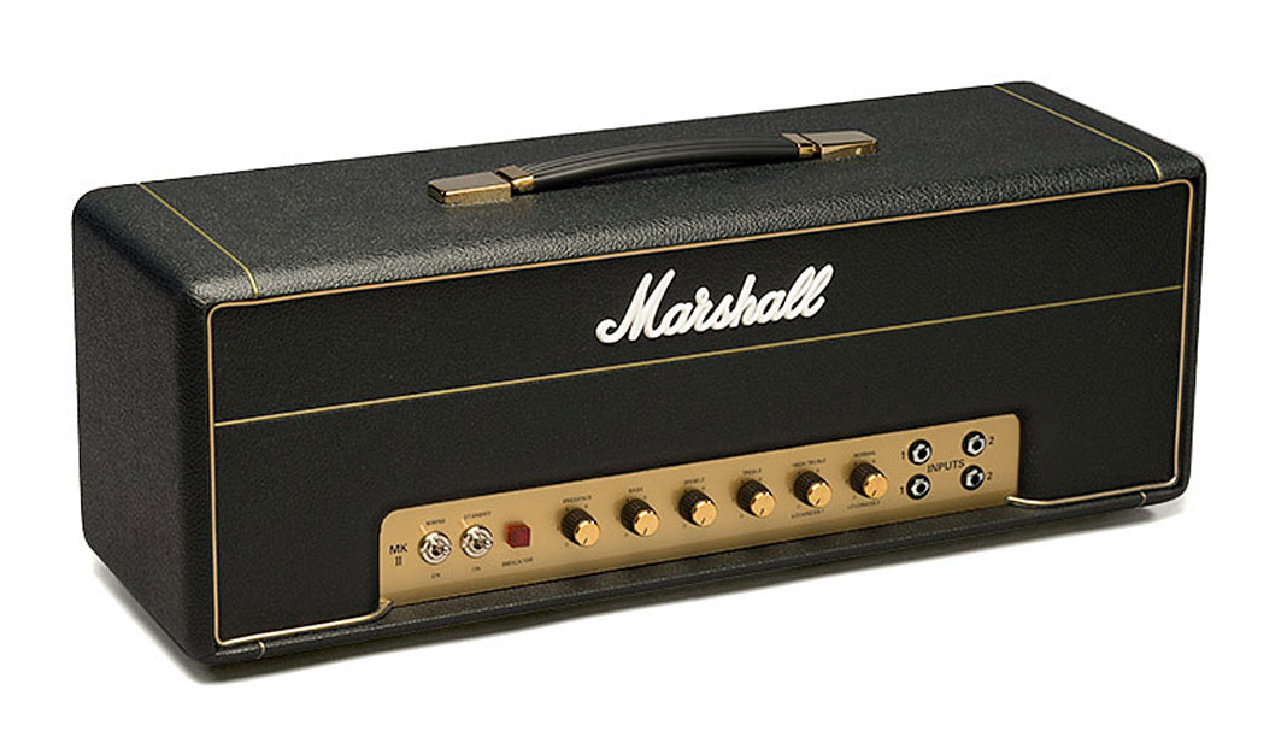
\includegraphics[scale=0.25]{1987x_head}
\caption{Guitar amplifiers, such as the classic Marshall 1987X head, are a good example of a multi-stage amplifier.  They usually have one or more gain stages available to give an overdriven and "crunchy" sound.}
\label{fig:ch15_intro}
\end{figure}
%%%%%%%%%%%%%%%%%%%%%%%%%%%%%%%%%%%%%%%%%%%%
\newpage
%%%%%%%%%%%%%%%%%%%%%%%%%%%%%%%%%%%%%%%%%%%%
%                 FIGURE                   %
%%%%%%%%%%%%%%%%%%%%%%%%%%%%%%%%%%%%%%%%%%%%
\begin{figure}[tb]
\centering
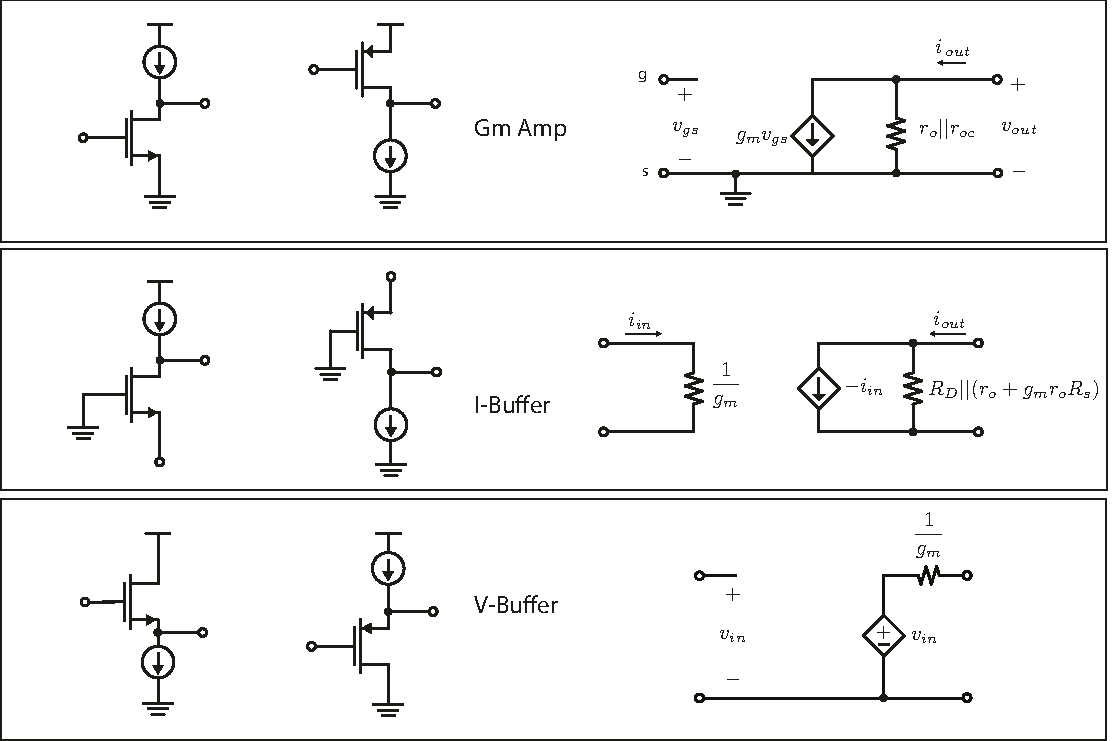
\includegraphics[width=\columnwidth]{ampchart_models}
\caption{Family of single-stage MOS transistor amplifiers and the two-port models.  This chart is important and should be committed to "memory".}
\label{fig:ampchart_models_fig}
\end{figure}
%%%%%%%%%%%%%%%%%%%%%%%%%%%%%%%%%%%%%%%%%%%%%%%%%%%%%%%%%%%%%%%%%%%%%%%%%%%%%%%%%%%%%%%%
%%%%%%%%%%%%%%%%%%%%%%%%%%%%%%%%%%%%%%%%%%%%%%%%%%%%%%%%%%%%%%%%%%%%%%%%%%%%%%%%%%%%%%%%
%                                   SECTION 15.2                                       %
%%%%%%%%%%%%%%%%%%%%%%%%%%%%%%%%%%%%%%%%%%%%%%%%%%%%%%%%%%%%%%%%%%%%%%%%%%%%%%%%%%%%%%%%
%%%%%%%%%%%%%%%%%%%%%%%%%%%%%%%%%%%%%%%%%%%%%%%%%%%%%%%%%%%%%%%%%%%%%%%%%%%%%%%%%%%%%%%%
\section{The Need for Multi-stage Amplifiers}
In the past few chapters, we have discussed single stage amplifiers in detail.  We have gone over building models for each type as either a voltage or current amplifier, or a hybrid amplifier (transconductance or transresistance).  See \emph{Fig.~\ref{fig:ampchart_models_fig}} for a reminder of these different topologies.  Why should we need to cascade single-stage amplifier stages?  The simplest reason is to provide more gain.   More is better, right? No, not always, but in the right circumstance, distributing gain over multiple stages has benefits. Such benefits include the ability to realize higher bandwidth, or for driving output loads without compromising the gain.  By separating the task of amplification into multiple steps, such as to drive an external load, we can better optimize each stage.\index{Amplifier!multi-stage}

To begin, let's talk about gain.  In modern technology, the amount of realizable gain per stage is limited, especially in nanoscale devices.  For example, in a technology with $L = 1\,\mu m$, a single device could provide an intrinsic gain $g_m\,r_o \approx 100$, whereas a short channel transistor in $28\,nm$ technology may only provide a gain of $10$.  

The other reason we use multiple amplifier stages is to \textit{better match the input and output source and load resistances to the amplifier}.  The source or load impedance may be too high or low, and a voltage or current buffer can often provide a better interface.  

Single stage amplifiers such as common source stages provide very high voltage gain.  But they suffer from low frequency poles, due to the lack of isolation from the input (gate) to the output (drain), flowing through the parasitic gate-drain capacitance $C_{gd}$.  Many multi-stage amplifiers improve the bandwidth by \textit{providing better isolation}.  

In other situations, an amplifier may have a high impedance node to provide large gain, and any additional capacitance on this node may be detrimental to bandwidth.  As we will see, \textit{a buffer can decouple the high impedance nodes from large load capacitors}.  

As mentioned earlier, output stages to drive "external" loads are often needed, and they usually have low gain owing to the fact that the load is a very small resistance (say a speaker or antenna).  Multiple gain stages are therefore required to isolate the load from the gain stages, and an output stage is needed to drive the load.  

Finally, more subtle applications of multi-stage amplification are for \textit{DC coupling}\index{Amplifier!DC coupling}, eliminating large passive elements such as capacitors that are needed to block the DC signal.   We can use amplifier stages to naturally \textbf{"level-shift"}\index{Amplifier!multi-stage!level-shifting} the signal.  Multi-stage amplifiers like \textit{differential stages} (covered in the next chapter) are also naturally more immune to the absolute DC level of the signal.  
%%%%%%%%%%%%%%%%%%%%%%%%%%%%%%%%%%%%%%%%%%%%%%%%%%%%%%%%%%%%%%%%%%%%%%%%%%%%%%%%%%%%%%%%
%%%%%%%%%%%%%%%%%%%%%%%%%%%%%%%%%%%%%%%%%%%%%%%%%%%%%%%%%%%%%%%%%%%%%%%%%%%%%%%%%%%%%%%%
%                                   SECTION 15.3                                       %
%%%%%%%%%%%%%%%%%%%%%%%%%%%%%%%%%%%%%%%%%%%%%%%%%%%%%%%%%%%%%%%%%%%%%%%%%%%%%%%%%%%%%%%%
%%%%%%%%%%%%%%%%%%%%%%%%%%%%%%%%%%%%%%%%%%%%%%%%%%%%%%%%%%%%%%%%%%%%%%%%%%%%%%%%%%%%%%%%
\section{Review Amplifier Input/Output Impedance Characteristics}
%%%%%%%%%%%%%%%%%%%%%%%%%%%%%%%%%%%%%%%%%%%%
%             SUBSECTION 15.3.1            %
%%%%%%%%%%%%%%%%%%%%%%%%%%%%%%%%%%%%%%%%%%%%
\subsection{Impedance "Match"}
On-chip circuits often use "voltage/current" matching to minimize loading.  Voltage matching means we drive a high impedance load with a low impedance source.  Current matching is the opposite, where we drive a low impedance load with a high impedance load.  This results in minimal signal attenuation.  At high frequencies, we can get even higher gain through passive element (resonant) matching gain circuits, but at lower frequencies the required values of inductance are not realizable or practical, especially on-chip.

\emph{Table~\ref{tab:imp}} level is a quick summary of the impedance levels of various ideal amplifier topologies and their input and output resistance levels.  For example, consider a voltage amplifier driving a current amplifier.  Since the current amplifier input impedance is low, and the voltage amplifier also has low output impedance, the cascade will suffer from loading effects.  However, if we cascade a voltage-to-current transconductance amplifier, we can see that the output/inputs are well suited to driving/load and all is well.
%%%%%%%%%%%%%%%%%%%%%%%%%%%%%%%%%%%%%%%%%%%%
%                 TABLE                    %
%%%%%%%%%%%%%%%%%%%%%%%%%%%%%%%%%%%%%%%%%%%%
\begin{table}[H]
\centering
\setlength{\tabcolsep}{20pt}
\renewcommand{\arraystretch}{1.5}
\begin{tabular}{|l|c|c|}
    \hline
    \textbf{Amplifier Type}  &  $R_{in}$ &  $R_{out}$\\
    \hline
    \textit{Voltage} & $\infty$ & $0$\\
    \hline
    \textit{Current} & $0$  &  $\infty$\\
    \hline
    \textit{Transconductance} & $\infty$ & $\infty$\\
    \hline
    \textit{Transresistance} & $0$ & $0$\\
    \hline
\end{tabular}
\caption{The input and output impedance of ideal amplifier types.
\label{tab:imp}} 
\end{table}
%%%%%%%%%%%%%%%%%%%%%%%%%%%%%%%%%%%%%%%%%%%%
\newpage
%%%%%%%%%%%%%%%%%%%%%%%%%%%%%%%%%%%%%%%%%%%%
%                 FIGURE                   %
%%%%%%%%%%%%%%%%%%%%%%%%%%%%%%%%%%%%%%%%%%%%
\begin{figure}[t]
\centering
\begin{tabular}{cc}
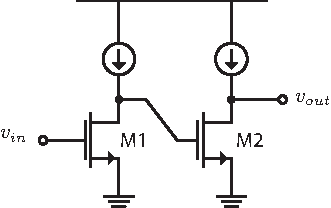
\includegraphics[scale=1.05]{cs_cascade_sch} &
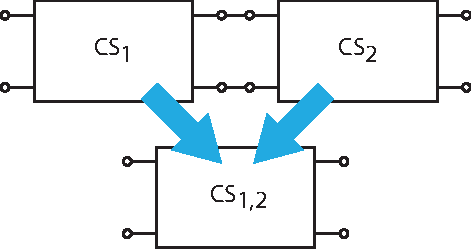
\includegraphics[width=.5\columnwidth]{1cascade}\\
(a) & (b)\\
\end{tabular}
\caption{(a) Cascade of two common-source stages.  (b) Cascading two stages can be considered as a composite single stage amplifier.}
\label{fig:1cascade}
\end{figure}
%%%%%%%%%%%%%%%%%%%%%%%%%%%%%%%%%%%%%%%%%%%%
%                 FIGURE                   %
%%%%%%%%%%%%%%%%%%%%%%%%%%%%%%%%%%%%%%%%%%%%
\begin{figure}[H]
\centering
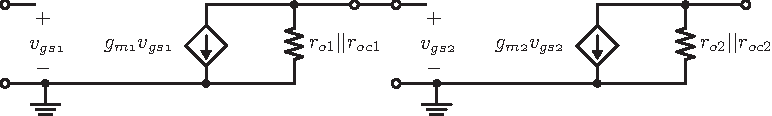
\includegraphics[scale=1.1]{2cs_casc_ss}
\caption{Low frequency small-signal schematic of a common-source cascade.}
\label{fig:2cs_casc_ss}
\end{figure}
%%%%%%%%%%%%%%%%%%%%%%%%%%%%%%%%%%%%%%%%%%%%%%%%%%%%%%%%%%%%%%%%%%%%%%%%%%%%%%%%%%%%%%%%
%%%%%%%%%%%%%%%%%%%%%%%%%%%%%%%%%%%%%%%%%%%%%%%%%%%%%%%%%%%%%%%%%%%%%%%%%%%%%%%%%%%%%%%%
%                                   SECTION 15.4                                       %
%%%%%%%%%%%%%%%%%%%%%%%%%%%%%%%%%%%%%%%%%%%%%%%%%%%%%%%%%%%%%%%%%%%%%%%%%%%%%%%%%%%%%%%%
%%%%%%%%%%%%%%%%%%%%%%%%%%%%%%%%%%%%%%%%%%%%%%%%%%%%%%%%%%%%%%%%%%%%%%%%%%%%%%%%%%%%%%%%
\section{Common-Source Cascades}
%%%%%%%%%%%%%%%%%%%%%%%%%%%%%%%%%%%%%%%%%%%%
%             SUBSECTION 15.4.1            %
%%%%%%%%%%%%%%%%%%%%%%%%%%%%%%%%%%%%%%%%%%%%
\subsection{Two-Stage Voltage Amplifier}
As shown in \emph{Fig.~\ref{fig:1cascade}}, simply cascading two amplifier stages is possible if the DC voltage levels are compatible. In other words, \textit{the desired operating point\index{Amplifier!operating point} of each individual amplifier should not change when we connect them}.  Otherwise, we would need AC coupling capacitors, but it is best to avoidusing them.  AC coupling capacitors\index{AC coupling capacitors} take up a lot of room on the chip or PCB, and they limit the range of operation (since they kill the low frequency gain).  For this reason, it is good to think of cascading amplifiers while designing them.  \textit{If we are careful to not disturb the operating points, the cascade will result in higher gain}.  We can think of the overall cascade as a single two-port model\index{Port models!two-port}.  If the amplifiers are unilateral, then the input impedance of the cascade is simply $R_{in} = R_{in,1}$, and the output impedance of the cascade is $R_{out} = R_{out,2}$.
%%%%%%%%%%%%%%%%%%%%%%%%%%%%%%%%%%%%%%%%%%%%
%             SUBSECTION 15.4.2            %
%%%%%%%%%%%%%%%%%%%%%%%%%%%%%%%%%%%%%%%%%%%%
\subsection{CS Cascade Analysis}
As an example of a cascade, let's take two common-source stages in cascade.  We need to ensure that the drain voltage of the first stage is the right bias point for the second stage gate.  Considering only the AC schematic shown in \emph{Fig.~\ref{fig:2cs_casc_ss}}, the resulting new \textit{two-port DC gain} can be analyzed by inspection:
    \begin{equation}
        A_v = \frac{v_{out}}{v_{in}} = -g_{m,1} \left(r_{o,1} \parallel r_{oc,1}\right)
                \cdot  -g_{m,2} \left(r_{o,2} \parallel r_{oc,2}\right)
        = \boxed{g_{m,1} \left(r_{o,1} \parallel r_{oc,1}\right) \cdot g_{m,2}\left(r_{o,2}||r_{oc,2}\right)}
    \end{equation}
The \textit{input impedance} is just the input impedance of the first stage:
    \begin{equation}
        R_{in} = R_{in,1} = \boxed{\infty\Omega}
    \end{equation} 
And the \textit{output impedance} is given by the second stage:
    \begin{equation}
        R_{out} = R_{out,2} = \boxed{r_{o,2} \parallel r_{oc,2}}
    \end{equation}
%%%%%%%%%%%%%%%%%%%%%%%%%%%%%%%%%%%%%%%%%%%%
\newpage
%%%%%%%%%%%%%%%%%%%%%%%%%%%%%%%%%%%%%%%%%%%%
%                 FIGURE                   %
%%%%%%%%%%%%%%%%%%%%%%%%%%%%%%%%%%%%%%%%%%%%
\begin{figure}[t]
\centering
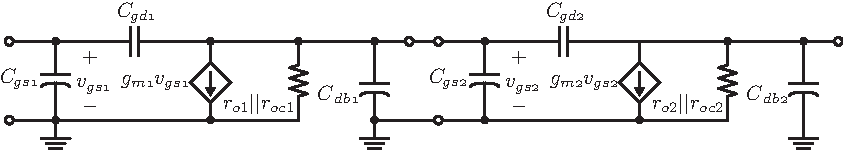
\includegraphics[scale=1.05]{3cs_casc_ss_cap}
\caption{AC small-signal schematic of a common-source cascade.}
\label{fig:3cs_casc_ss_cap}
\end{figure}
%%%%%%%%%%%%%%%%%%%%%%%%%%%%%%%%%%%%%%%%%%%%
%             SUBSECTION 15.4.3            %
%%%%%%%%%%%%%%%%%%%%%%%%%%%%%%%%%%%%%%%%%%%%
\subsection{CS Cascade Frequency Response}
The AC schematic shown in \emph{Fig.~\ref{fig:3cs_casc_ss_cap}} looks complicated, with six capacitors shown.  But if we combine parallel components and also apply the Miller theorem\index{Miller's theorem}, we can identify three independent nodes.  At the input, applying Miller's theorem:
    \begin{equation} 
        C_{M_1} = C_{gs,1} + C_{gd,1} (1 - A_{v_1})
    \end{equation}
We can approximate the gain of the first stage:
    \begin{equation} 
        A_{v_1} = -g_{m,1} r_{o,1} \parallel r_{oc,1}
    \end{equation}
This results in a composite capacitance of:
    \begin{equation} 
        C_{M_1} = C_{gs,1} + C_{gd,1} (1 + g_{m,1} r_{o,1} \parallel r_{oc,1})
    \end{equation}
The second stage is exactly the same, starting with the Miller capacitance:
    \begin{equation} 
        C_{M_2} = C_{gs,2} + C_{db,1} + C_{gd,2} (1 - A_{v_2})
    \end{equation}
Approximating the gain:
    \begin{equation} 
        A_{v_2} = -g_{m,2} (r_{o,2} \parallel r_{oc,2})
    \end{equation}
Results in a second Miller composite capacitance:
    \begin{equation} 
        C_{M_2} = C_{gs,2} + C_{db,1} + C_{gd,2} (1 + g_{m,2} r_{o,2} \parallel r_{oc,2})
    \end{equation}
The simplified schematic is shown in \emph{Fig.~\ref{fig:4cs_casc_ss_cap_miller}}.  The time constant of the input node is given by:
    \begin{equation}
        \tau_1 = C_{M_1}\,R_s
    \end{equation}
and the intermediate node is given by:
    \begin{equation} 
        \tau_2 = C_{M_2}(r_{o,1} \parallel r_{oc,1})
    \end{equation}
Notice that $\tau_1$ depends on the source resistance $R_s$, which can be lowered to improve the bandwidth.  On the other hand,  the intermediate node is a killer, because the resistance is large (output resistance of transistors), and the capacitance is large due to Miller multiplication.  The output may also contribute a pole, especially if driving a capacitive load.  Many poles results in very poor bandwidth, especially if they are all close in magnitude.  This is one of the main issues with the multi-stage common-source cascade.
%%%%%%%%%%%%%%%%%%%%%%%%%%%%%%%%%%%%%%%%%%%%
%                 FIGURE                   %
%%%%%%%%%%%%%%%%%%%%%%%%%%%%%%%%%%%%%%%%%%%%
\begin{figure}[H]
\centering
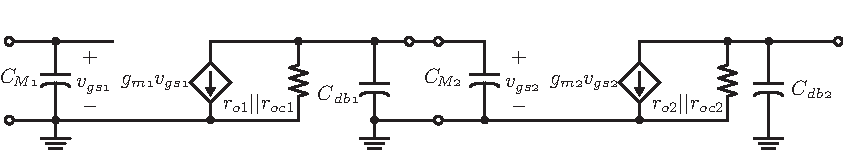
\includegraphics[scale=1.05]{4cs_casc_ss_cap_miller}
\caption{Simplified small-signal schematic of a common-source cascade using the Miller approximations.}
\label{fig:4cs_casc_ss_cap_miller}
\end{figure}
%%%%%%%%%%%%%%%%%%%%%%%%%%%%%%%%%%%%%%%%%%%%
\newpage
%%%%%%%%%%%%%%%%%%%%%%%%%%%%%%%%%%%%%%%%%%%%
%                 FIGURE                   %
%%%%%%%%%%%%%%%%%%%%%%%%%%%%%%%%%%%%%%%%%%%%
\begin{figure}[t]
\centering
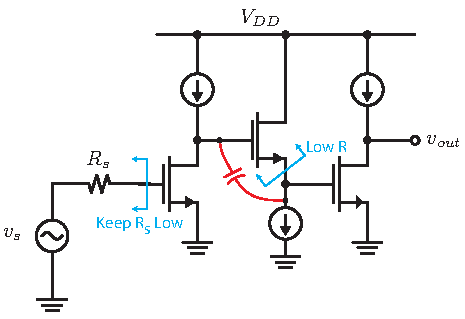
\includegraphics[scale=1.35]{55cs_cd_cs_casc}
\caption{Common-source cascade with an internal source follower buffer to improve the bandwidth.}
\label{fig:55cs_cd_cs_casc}
\end{figure}
%%%%%%%%%%%%%%%%%%%%%%%%%%%%%%%%%%%%%%%%%%%%
%                 FIGURE                   %
%%%%%%%%%%%%%%%%%%%%%%%%%%%%%%%%%%%%%%%%%%%%
\begin{figure}[H]
\centering
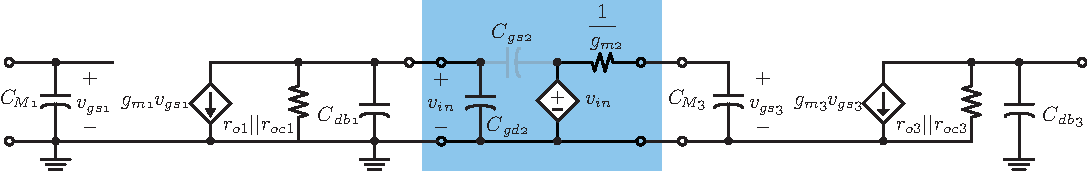
\includegraphics[width=\columnwidth]{5cs_cd_cs_casc_ss_miller}
\caption{Small-signal model of common-source cascade with internal source follower buffer (highlighted).}
\label{fig:5cs_cd_cs_casc_ss_miller}
\end{figure}
%%%%%%%%%%%%%%%%%%%%%%%%%%%%%%%%%%%%%%%%%%%%
%             SUBSECTION 15.4.4            %
%%%%%%%%%%%%%%%%%%%%%%%%%%%%%%%%%%%%%%%%%%%%
\subsection{Bandwidth Extension}
The common source stage has high gain, but it suffers from a low bandwidth.  A follower stage can buffer the Miller cap from the high output impedance of a second transistor, because it has low output impedance ($\frac{1}{g_m}$), as shown in \emph{Fig.~\ref{fig:55cs_cd_cs_casc}}.  We still need to keep $R_s$ under control.  Recall that the $C_{gs}$ of the follower stage is \textit{"bootstrapped"}\index{Amplifier!bootstrapping}, and it does not load the common source stage:
    \begin{equation}
    	C_M = C_{gs} (1 - A_v) \approx 0\,F
    \end{equation}
As shown in \emph{Fig.~\ref{fig:5cs_cd_cs_casc_ss_miller}}, for the input time constant, we have (as before):   
    \begin{equation} 
        \tau_1 = \Big(C_{gs,1} + C_{gd,1} (1 + g_{m,1} r_{o,1} \parallel r_{oc,1})\Big)\,R_s
    \end{equation}
For the input of the follower, the capacitance is low because of the follower bootstrapping:
    \begin{equation} 
        \tau_2 = (C_{db,1} + C_{gd,2})\,r_{o,1} \parallel r_{oc,1}
    \end{equation}
At the output of the buffer, the low output impedance keeps the time constant small:
    \begin{equation}  
        \tau_3 = \Big(C_{gs,3} + C_{gd,3} (1 + g_{m,3}\,r_{o,3} \parallel r_{oc,3})\Big)\left(\frac{1}{g_{m,2}}\right)
    \end{equation}
At the load, if there is no load capacitance, we have another relatively high frequency pole:
    \begin{equation}  
        \tau_4 = C_{db,3}\,(r_{o,3} \parallel r_{oc,3})
    \end{equation}
\newpage
%%%%%%%%%%%%%%%%%%%%%%%%%%%%%%%%%%%%%%%%%%%%
%                 FIGURE                   %
%%%%%%%%%%%%%%%%%%%%%%%%%%%%%%%%%%%%%%%%%%%%
\begin{figure}[tb]
\centering
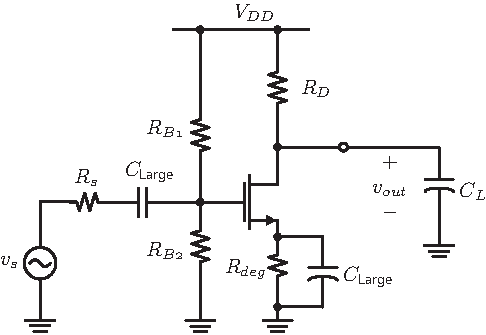
\includegraphics[scale=1.35]{6cs_dc}
\caption{Complete schematic of a common-source amplifier including DC biasing elements.}
\label{fig:6cs_dc}
\end{figure}
%%%%%%%%%%%%%%%%%%%%%%%%%%%%%%%%%%%%%%%%%%%%
%                 FIGURE                   %
%%%%%%%%%%%%%%%%%%%%%%%%%%%%%%%%%%%%%%%%%%%%
\begin{figure}[H]
\centering
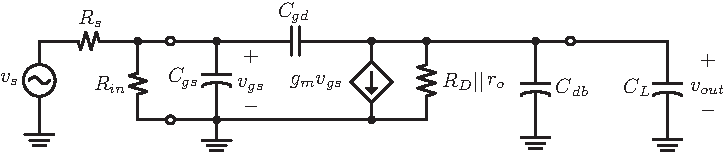
\includegraphics[scale=1.20]{7cs_cL_ss}
\caption{AC small-signal schematic of common-source amplifier including the effective loading by biasing elements $R_{in}$. and load capacitor $C_L$.}
\label{fig:7cs_cL_ss}
\end{figure}
%%%%%%%%%%%%%%%%%%%%%%%%%%%%%%%%%%%%%%%%%%%%%%%%%%%%%%%%%%%%%%%%%%%%%%%%%%%%%%%%%%%%%%%%
%%%%%%%%%%%%%%%%%%%%%%%%%%%%%%%%%%%%%%%%%%%%%%%%%%%%%%%%%%%%%%%%%%%%%%%%%%%%%%%%%%%%%%%%
%                                   SECTION 15.5                                       %
%%%%%%%%%%%%%%%%%%%%%%%%%%%%%%%%%%%%%%%%%%%%%%%%%%%%%%%%%%%%%%%%%%%%%%%%%%%%%%%%%%%%%%%%
%%%%%%%%%%%%%%%%%%%%%%%%%%%%%%%%%%%%%%%%%%%%%%%%%%%%%%%%%%%%%%%%%%%%%%%%%%%%%%%%%%%%%%%%
\section{Common-Source with Capacitive Load}
%%%%%%%%%%%%%%%%%%%%%%%%%%%%%%%%%%%%%%%%%%%%
%             SUBSECTION 15.5.1            %
%%%%%%%%%%%%%%%%%%%%%%%%%%%%%%%%%%%%%%%%%%%%
\subsection{Common-Source with a Large Capacitive Load}
A schematic of a common source amplifier with biasing elements is shown in \emph{Fig.~\ref{fig:6cs_dc}}. Recall that $C_{\text{Large}}$ is a very large bypass capacitor\index{Capacitor!bypass}.  Usually these capacitors function better the larger they get, because they define the low frequency cutoff limit.  These capacitors look like short circuits to the AC signal.  On the other hand, if the load capacitance $C_L$ is large, its pole dominates. Let's analyze this scenario.

In \emph{Fig.~\ref{fig:7cs_cL_ss}}, note that $R_{in}$ represents the parallel combination of the biasing resistors, $R_{in} = R_{B1} || R_{B2}$.  If we make a Miller approximation, the input time constant is given by:
    \begin{equation}
        \tau_1 = \left(R_s \parallel R_{in}\right)\,\Big(C_{gs} + g_m \left(r_o \parallel R_D\right) C_{gd}\Big)
    \end{equation}
At the output, we have a large capacitor $C_L \gg C_{gs,gd,db}$, so it dominates the time constant over the transistor parasitics:
    \begin{equation}
        \tau_2 \approx \left(R_D \parallel r_o\right)\,C_L
    \end{equation}
\newpage
%%%%%%%%%%%%%%%%%%%%%%%%%%%%%%%%%%%%%%%%%%%%
%                 FIGURE                   %
%%%%%%%%%%%%%%%%%%%%%%%%%%%%%%%%%%%%%%%%%%%%
\begin{figure}[t]
\centering
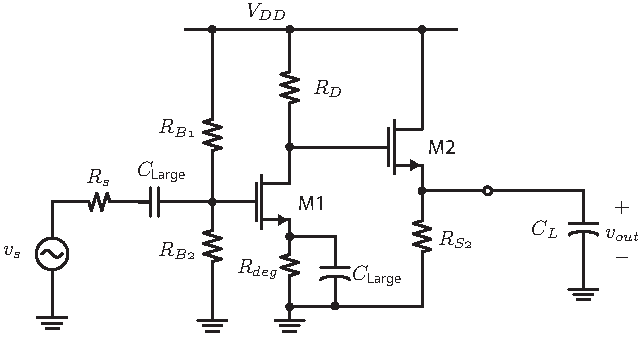
\includegraphics[scale=1.35]{8_cs_cd_casc_dc}
\caption{Common-drain (follower) buffer added to the common-source amplifier aids in driving a large capacitive load $C_L$.}
\label{fig:8_cs_cd_casc_dc}
\end{figure}
%%%%%%%%%%%%%%%%%%%%%%%%%%%%%%%%%%%%%%%%%%%%
\vspace{1cm}
What can we do if we have to drive a large capacitive load, $C_L$?  How can we reduce the impact of $C_L$? One way is to reduce the resistance $R_D$.  However, increasing $R_D$ reduces our pass-band gain.  To recover the gain we can increase $g_{m,1}$.  But this comes at the cost of increased power consumption.  There is a better way to extend the bandwidth, which is to add a source follower stage.  This is illustrated in \emph{Fig.~\ref{fig:8_cs_cd_casc_dc}}.  Adding the source follower stage allows us to buffer the output load capacitor from the gain stage.

The analysis is similar to previous example.  As shown in the AC schematic in \emph{Fig.~\ref{fig:9cs_cd_casc_ss}}, by adding a common-drain stage (Source Follower), we can increase the bandwidth. Even though it costs us power for the follower stage, increasing the bandwidth by increasing $g_{m1}$ costs us much more.
\vspace{1cm}
%%%%%%%%%%%%%%%%%%%%%%%%%%%%%%%%%%%%%%%%%%%%
%                 FIGURE                   %
%%%%%%%%%%%%%%%%%%%%%%%%%%%%%%%%%%%%%%%%%%%%
\begin{figure}[H]
\centering
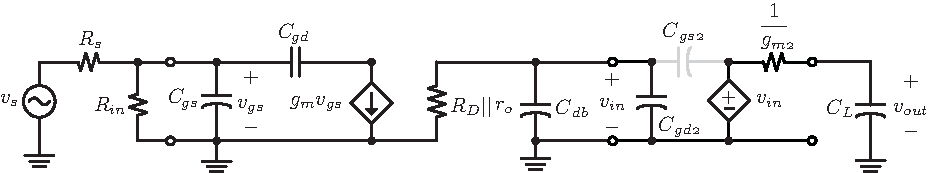
\includegraphics[scale=0.95]{9cs_cd_casc_ss}
\caption{AC small-signal model of a common-source / common-drain cascade.}
\label{fig:9cs_cd_casc_ss}
\end{figure}
%%%%%%%%%%%%%%%%%%%%%%%%%%%%%%%%%%%%%%%%%%%%
\newpage
%%%%%%%%%%%%%%%%%%%%%%%%%%%%%%%%%%%%%%%%%%%%
%                 FIGURE                   %
%%%%%%%%%%%%%%%%%%%%%%%%%%%%%%%%%%%%%%%%%%%%
\begin{figure}[t]
\centering
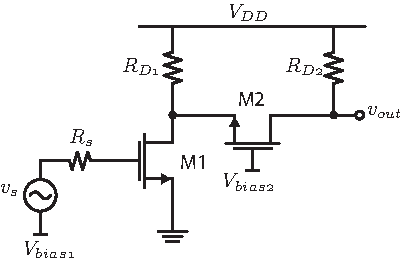
\includegraphics[scale=1.25]{10cs_cg_cascade}
\caption{Common-source stage followed by a common-gate stage.}
\label{fig:10cs_cg_cascade}
\end{figure}
%%%%%%%%%%%%%%%%%%%%%%%%%%%%%%%%%%%%%%%%%%%%
%                 FIGURE                   %
%%%%%%%%%%%%%%%%%%%%%%%%%%%%%%%%%%%%%%%%%%%%
\begin{figure}[H]
\centering
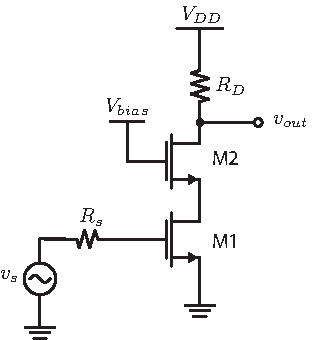
\includegraphics[scale=1.25]{10cascode_dc}
\caption{A stacked common-source stage followed by a common-gate stage, known as a "cascode" amplifier.}
\label{fig:10cascode_dc}
\end{figure}
%%%%%%%%%%%%%%%%%%%%%%%%%%%%%%%%%%%%%%%%%%%%%%%%%%%%%%%%%%%%%%%%%%%%%%%%%%%%%%%%%%%%%%%%
%%%%%%%%%%%%%%%%%%%%%%%%%%%%%%%%%%%%%%%%%%%%%%%%%%%%%%%%%%%%%%%%%%%%%%%%%%%%%%%%%%%%%%%%
%                                   SECTION 15.6                                       %
%%%%%%%%%%%%%%%%%%%%%%%%%%%%%%%%%%%%%%%%%%%%%%%%%%%%%%%%%%%%%%%%%%%%%%%%%%%%%%%%%%%%%%%%
%%%%%%%%%%%%%%%%%%%%%%%%%%%%%%%%%%%%%%%%%%%%%%%%%%%%%%%%%%%%%%%%%%%%%%%%%%%%%%%%%%%%%%%%
\section{Common-Source Common-Gate Cascade (Cascode)}
%%%%%%%%%%%%%%%%%%%%%%%%%%%%%%%%%%%%%%%%%%%%
%             SUBSECTION 15.6.1            %
%%%%%%%%%%%%%%%%%%%%%%%%%%%%%%%%%%%%%%%%%%%%
\subsection{The Common-Source / Common-Gate Cascade}
Consider the cascade shown in \emph{Fig.~\ref{fig:10cs_cg_cascade}}.  The common source stage provides gain, and the common gate acts as a current buffer, passing the current to the load.  Since the current buffer stage has a gain of one, is it even helping?  On first pass, it seems like $M2$ is not doing anything, because it just buffers the current of $M1$ and does not provide gain.  But understanding this topology is more subtle as it provides potential gain and bandwidth benefits.
%%%%%%%%%%%%%%%%%%%%%%%%%%%%%%%%%%%%%%%%%%%%
%             SUBSECTION 15.6.2            %
%%%%%%%%%%%%%%%%%%%%%%%%%%%%%%%%%%%%%%%%%%%%
\subsection{Merged CS + CG = Cascode}
As seen in \emph{Fig.~\ref{fig:10cascode_dc}}, we can share the bias currents between the two amplifier stages by stacking them into a common structure, commonly known as a \textbf{cascode}\index{Amplifier!multi-stage!cascode}\index{Amplifier!types!cascode}.  While this circuit has \textit{reduced headroom}\index{Amplifier!headroom}, it can be seen as a "supercharged" common source stage.  We know that the $g_m$ of the combined $M1$/$M2$ amplifier is the same as a single transistor, but the output impedance is boosted by the $g_m\,r_o$ of the transistor.
\newpage
%%%%%%%%%%%%%%%%%%%%%%%%%%%%%%%%%%%%%%%%%%%%
%                 FIGURE                   %
%%%%%%%%%%%%%%%%%%%%%%%%%%%%%%%%%%%%%%%%%%%%
\begin{figure}[t]
\centering
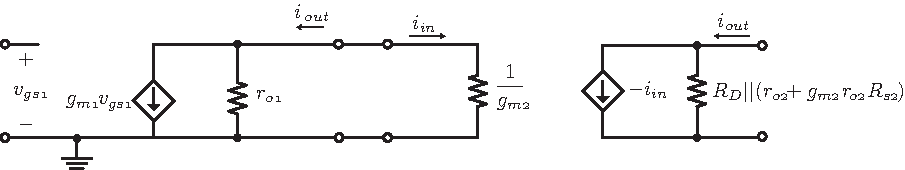
\includegraphics[scale=0.98]{11cascode_ss}
\caption{Small-signal model of the cascode amplifier.}
\label{fig:11cascode_ss}
\end{figure}
%%%%%%%%%%%%%%%%%%%%%%%%%%%%%%%%%%%%%%%%%%%%
%             SUBSECTION 15.6.3            %
%%%%%%%%%%%%%%%%%%%%%%%%%%%%%%%%%%%%%%%%%%%%
\subsection{Cascode Gain}
Let's apply two-port small-signal analysis, shown in \emph{Fig.~\ref{fig:11cascode_ss}}.  Note the common gate stage is degenerated by $M1$, so $R_{s,2} = r_{o,1}$. In this case, we care about the \textit{input current }to the second stage. Since the input resistance of the CG is low, the majority of the CS current is fed to the CG stage.  This means the DC gain of the amplifier is given by:
    \begin{equation}
        A_v = -g_{m,1}\Big(R_D \parallel (r_{o,2} + g_{m,2}\,r_{o,2}\,r_{o,1})Big) \boxed{\approx -g_{m,1}\,R_D}
    \end{equation}
This is no better than a common-source stage?  So why use a cascode?  Well, for one you can immediately see that we are throwing away a lot of gain by using $R_D$.  If we instead use an ideal current source, the gain will rise to:
    \begin{equation}
        A_v = -g_{m,1}\left(r_{o,2} + g_{m,2}\,r_{o,2}\,r_{o,1}\right) \boxed{\approx -{(g_m\,r_o)}^2}
    \end{equation}
This is substantially higher than the maximum gain of a single transistor, giving credence to the "supercharged" transistor claim.  But it is even better than that when we consider bandwidth. 
%%%%%%%%%%%%%%%%%%%%%%%%%%%%%%%%%%%%%%%%%%%%
%             SUBSECTION 15.6.4            %
%%%%%%%%%%%%%%%%%%%%%%%%%%%%%%%%%%%%%%%%%%%%
\subsection{Cascode Bandwidth}
To analyze the bandwidth of the cascade, let's add all the transistor parasitic capacitors, as shown in \emph{Fig.~\ref{fig:12cascode_caps}a}.  Notice that with all the parasitic capacitors in this circuit, our first step is try to combine as many as possible.   Let's identify three key nodes in the circuit: the gate \emph{g}, the internal node at the drain of $M1$ labeled \emph{i}, and the output labeled \emph{o}, shown in \emph{Fig.~\ref{fig:12cascode_caps}b}.  Next, we can apply Miller's theorem\index{Miller's theorem} to get a sense for the bandwidth limiting stages.  We immediately notice a difference in the Miller capacitance.  For $M2$, its $C_{gd}$ is simply grounded, and it is \textit{not} Miller multiplied.  On the other hand, for $M1$, the Miller capacitance is "shielded" from the high voltage gain at the output node.  We will also show that the voltage gain experienced at the intermediate node is much lower.  
%%%%%%%%%%%%%%%%%%%%%%%%%%%%%%%%%%%%%%%%%%%%
%                 FIGURE                   %
%%%%%%%%%%%%%%%%%%%%%%%%%%%%%%%%%%%%%%%%%%%%
\begin{figure}[H]
\centering
\begin{tabular}{cc}
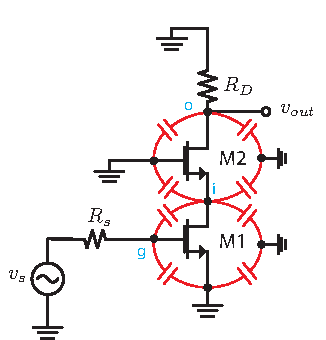
\includegraphics[scale=0.96]{12cascode_caps} &
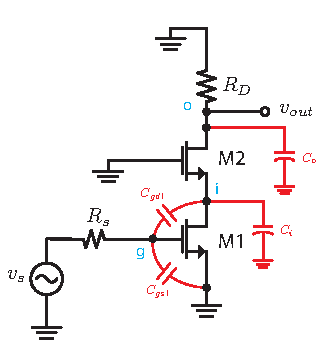
\includegraphics[scale=0.96]{13cascode_caps_simple}\\
(a) & (b)\\
\end{tabular}
\caption{(a) Cascode amplifier with capacitive transistor parasitics.  (b) Simplified schematic obtained by keeping only the relevant capacitors and combining the others.}
\label{fig:12cascode_caps}
\end{figure}
%%%%%%%%%%%%%%%%%%%%%%%%%%%%%%%%%%%%%%%%%%%%
\newpage
%%%%%%%%%%%%%%%%%%%%%%%%%%%%%%%%%%%%%%%%%%%%
%                 FIGURE                   %
%%%%%%%%%%%%%%%%%%%%%%%%%%%%%%%%%%%%%%%%%%%%
\begin{figure}[t]
\centering
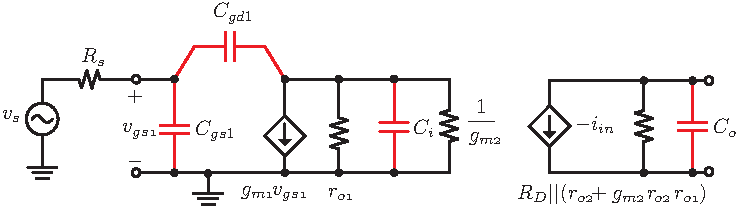
\includegraphics[scale=1.15]{14cascode_ac_ss}
\caption{Small-signal model of a cascode amplifier using the two-port common-gate model.} \label{fig:14cascode_ac_ss}
\end{figure}
%%%%%%%%%%%%%%%%%%%%%%%%%%%%%%%%%%%%%%%%%%%%
%             SUBSECTION 15.6.5            %
%%%%%%%%%%%%%%%%%%%%%%%%%%%%%%%%%%%%%%%%%%%%
\subsection{Cascode Bandwidth - Small Signal}
For a complete analysis of the bandwidth of the cascode amplifier, let's examine the small-signal model, shown in \emph{Fig.~\ref{fig:14cascode_ac_ss}}.  Notice that we take advantage of the equivalent two-port circuit model of the common gate stage.   At the input node, $C_{gd,1}$ is Miller multiplied like a common source, but we need to find the voltage gain from the gate to the drain of $M1$.  This is given by:
    \begin{equation}
        A_{v_i} = \frac{v_i}{v_g} = -g_{m,1} \left( r_{o,1} \parallel \frac{1}{g_{m,2}} \right) \approx \frac{-g_{m,1}}{g_{m,2}}
    \end{equation}
Since $M1$ and $M2$ share the same current, if they are sized equally, the internal voltage gain is simply $A_{v_i} = -1$.  Then the Miller multiplication is small:
    \begin{equation}
        \tau_g = R_s\,(C_{gs,1} + 2\,C_{gd,1})
    \end{equation}
The intermediate node is a wide bandwidth node, because the common gate amplifier has a low input impedance of $\frac{1}{g_{m,2}}$:
    \begin{equation}
        \tau_i = C_i\left(\frac{1}{g_{m,2}} \parallel r_{o,1}\right) \approx \frac{C_i}{g_{m,2}}
    \end{equation}  
Finally, the output node bandwidth depends on the load and $R_D$:
    \begin{equation}
        \tau_o = C_o\,(R_D \parallel (r_{o,2} + g_{m,2}\,r_{o,2}\,r_{o,1})) \approx R_D\,C_o
    \end{equation}
We now can appreciate the benefits of the cascode amplifier.  It is essentially a supercharged transistor with the same $g_m$, but it does not suffer from the Miller effect (as much), and the achievable gain is much higher.  For this reason, the cascode is a workhorse gain stage used in many amplifiers.  The only down side is the reduced voltage headroom, discussed in the next section.
\newpage
%%%%%%%%%%%%%%%%%%%%%%%%%%%%%%%%%%%%%%%%%%%%
%                 FIGURE                   %
%%%%%%%%%%%%%%%%%%%%%%%%%%%%%%%%%%%%%%%%%%%%
\begin{figure}[tb]
\centering
\begin{tabular}{cc}
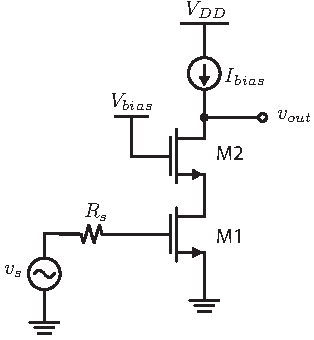
\includegraphics[scale=1.35]{15cascode_current_source_dc} &
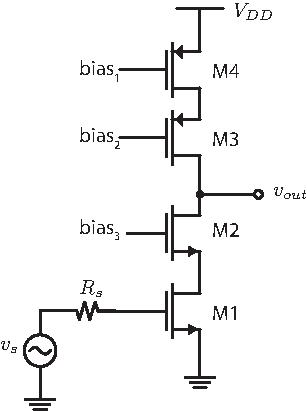
\includegraphics[scale=1.15]{cascode_current_load_cascode.pdf}\\
(a) & (b)\\
\end{tabular}
\caption{(a) A high gain cascode amplifier biased with an ideal current source $I_{bias}$.  (b) The ideal current source load is replaced with a cascode load to maximize the gain.}  \label{fig:15cascode_current_source_dc}
\end{figure}
%%%%%%%%%%%%%%%%%%%%%%%%%%%%%%%%%%%%%%%%%%%%
%             SUBSECTION 15.6.6            %
%%%%%%%%%%%%%%%%%%%%%%%%%%%%%%%%%%%%%%%%%%%%
\subsection{Cascode Biasing}
As discussed previously, the output impedance of the cascode is very high, and loading it with $R_D$ is likely to reduce the voltage gain.  The best we can do is to use a current source load, shown in \emph{Fig.~\ref{fig:15cascode_current_source_dc}a}, but $r_{oc}$ needs to be very large. Thus, we should use a cascode current mirror load as shown in \emph{Fig.~\ref{fig:15cascode_current_source_dc}b}.
%%%%%%%%%%%%%%%%%%%%%%%%%%%%%%%%%%%%%%%%%%%%
%             SUBSECTION 15.6.7            %
%%%%%%%%%%%%%%%%%%%%%%%%%%%%%%%%%%%%%%%%%%%%
\subsection{Example:  Complete Amplifier Design}
Let's design a complete cascode amplifier with the following goal of achieving a DC gain magnitude of $5000$.   Let's choose $g_{m,1} = 1\,mS$.\footnote{In \emph{Ch.~\ref{ch:ch17_opamps_fb}}, we'll see that a given value of $g_m$ is needed for the transconductance stage to meet bandwidth specs.} For simplicity, we will assume that all of the $g_m$ and $r_o$ values are equal.  Since the gain is given by:
    \begin{equation} 
        {A_v} \approx - g_{m,1}\,R_{out} = -1\,mS \cdot 5\,M\Omega = \boxed{-5000}
    \end{equation}
The required output resistance is given by:
    \begin{equation} 
        R_{out} \approx \left(\frac{1}{2}\right)g_m\,r_o^2 = \boxed{5\,M\Omega}
    \end{equation}
The factor of one half accounts for the parallel combination of the $NMOS$ and $PMOS$ cascode stages.  One for the cascode amplifier, and the other the cascode mirror load.  That means each transistor needs an output resistance $r_o$ of:
    \begin{equation} 
        r_o = \sqrt{\frac{20\,M\Omega}{g_m}}
        = \sqrt{\frac{10\,M\Omega}{1\,mS}} = \boxed{100\,k\Omega}
    \end{equation}
\newpage
%%%%%%%%%%%%%%%%%%%%%%%%%%%%%%%%%%%%%%%%%%%%
%              SUB-SUBSECTION              %
%%%%%%%%%%%%%%%%%%%%%%%%%%%%%%%%%%%%%%%%%%%%
\subsubsection{Bias Current and Device Sizing}
To complete the design, we need to know process parameters to solve for $\frac{W}{L}$.  We are given the following technology parameters: $k = \mu\,C_{ox} = 100\,\mu A/V^2$ and $\lambda = .1V^{-1}$.  With knowledge of these parameters, we can calculate the DC current:
    \begin{equation}
        r_o = \frac{1}{\lambda\,I_{DS}} = \boxed{100\,k\Omega}
    \end{equation}
    \begin{equation}
        I_{DS} = \frac{1}{0.1\,V^{-1} \cdot 100\,k\Omega} = \boxed{100\,\mu A}
    \end{equation}
Since we have specified the $g_m$, we can now find the device size $\frac{W}{L}$:
    \begin{equation} 
        g_m = \sqrt{2k\left(\frac{W}{L}\right) {I_{DS}}} = \boxed{1\,mS}
    \end{equation}
    \begin{equation} 
        \frac{W}{L} = \frac{{g_m}^2}{2k\,I_{DS}}
        = \frac{{(1\,mS)}^2}{2 \cdot 100\,\mu \cdot 100\,\mu A} = \boxed{50}
    \end{equation}
You may question our selection of $g_m$, which implies the DC current and device dimensions.  The reason we pre-selected $g_m$ is related to the fact that we desire a certain gain bandwidth in amplifiers, a topic which we will cover when we discuss op-amps.  For now, simply accept it as a given that amplifiers need a minimum $g_m$ in certain cases to meet specifications that we have not discussed.
%%%%%%%%%%%%%%%%%%%%%%%%%%%%%%%%%%%%%%%%%%%%
%              SUB-SUBSECTION              %
%%%%%%%%%%%%%%%%%%%%%%%%%%%%%%%%%%%%%%%%%%%%
\subsubsection{Output (Voltage) Swing}
The biggest downside to this enormous cascode amplifier is the low voltage swing\index{Voltage swing}.  Recall that each transistor operates with a certain overdrive voltage\index{MOSFET!overdrive voltage} related to the current, which is also known as the $V_{d,sat}$ of a transistor:
    \begin{equation}
        V_{OD} = V_T + \sqrt{\frac{2\,I_{DS}}{\mu\,C_{ox}\frac{W}{L}}}
    \end{equation}
For our example:
    \begin{equation} 
        g_m = \frac{2\,I_{DS}}{V_{GS} - V_T} = \boxed{1\,mS}
    \end{equation}
This leads to:
    \begin{equation}
        V_{GS} - V_T = \frac{2\,I_{DS}}{g_m} = \frac{2 \cdot 100\,\mu A}{1\,mS} = \boxed{0.2\,V}
    \end{equation}
For long channel devices, this is simply $V_{GS} - V_T$.  To keep all devices in saturation, we have to ensure that the voltage levels don not exceed the following limits:
    \begin{align}
        V_o &< V_{DD} - 2\,V_{OD}\\
        V_o &> 2\,V_{OD}
    \end{align} 
That means that the minimum supply voltage is $V_{swing} + (0.2\,V \cdot 4) = 0.8,V + V_{swing}$.  For example, for a $0.4\,V$ swing, we need at least $1.2\,V$.  

One issue we have been avoiding is how we would actually deliver all the bias voltages shown in \emph{Fig.~\ref{fig:15cascode_current_source_dc}b}.  The input transistor needs a bias to establish the current, but we need to ensure this current matches the top $PMOS$ transistor.  In fact, this is the major problem with this circuit, because the cascode $M1$ will "fight" the cascode current mirror load $M4$ to establish the current, resulting in an undetermined DC output level.  In practice, we need a feedback circuit to establish a well defined output voltage that does not vary with temperature, process, and supply voltage.  In other words, we need to program the gate voltage of $M4$ (labeled bias$_1$) to achieve the desired output DC level (say mid-rail).
\newpage
%%%%%%%%%%%%%%%%%%%%%%%%%%%%%%%%%%%%%%%%%%%%
%                 FIGURE                   %
%%%%%%%%%%%%%%%%%%%%%%%%%%%%%%%%%%%%%%%%%%%%
\begin{figure}[t]
\centering
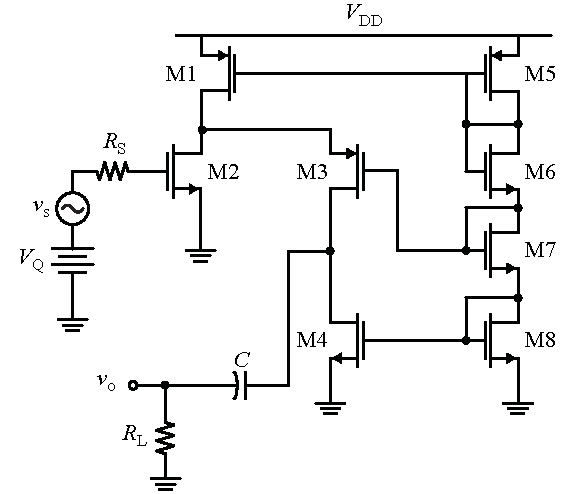
\includegraphics[scale=0.85]{16cascode_folded}
\caption{A "big" example to be analyzed in a step-by-step fashion.}
\label{fig:16cascode_folded}
\end{figure}
%%%%%%%%%%%%%%%%%%%%%%%%%%%%%%%%%%%%%%%%%%%%%%%%%%%%%%%%%%%%%%%%%%%%%%%%%%%%%%%%%%%%%%%%
%%%%%%%%%%%%%%%%%%%%%%%%%%%%%%%%%%%%%%%%%%%%%%%%%%%%%%%%%%%%%%%%%%%%%%%%%%%%%%%%%%%%%%%%
%                                   SECTION 15.7                                       %
%%%%%%%%%%%%%%%%%%%%%%%%%%%%%%%%%%%%%%%%%%%%%%%%%%%%%%%%%%%%%%%%%%%%%%%%%%%%%%%%%%%%%%%%
%%%%%%%%%%%%%%%%%%%%%%%%%%%%%%%%%%%%%%%%%%%%%%%%%%%%%%%%%%%%%%%%%%%%%%%%%%%%%%%%%%%%%%%%
\section{"Big Circuit" Example}
Let's end this chapter by bringing together all the various concepts to analyze a "big" circuit, shown in \emph{Fig.~\ref{fig:16cascode_folded}}.  At first it looks intimidating, but we will solve this problem one step at a time.
%%%%%%%%%%%%%%%%%%%%%%%%%%%%%%%%%%%%%%%%%%%%
%             SUBSECTION 15.7.1            %
%%%%%%%%%%%%%%%%%%%%%%%%%%%%%%%%%%%%%%%%%%%%
\subsection{Cutting Through the Complexity}
The key to analyzing a big circuit is to cut out all the clutter.  To do this, identify the "signal path" between the input and output, and aggressively eliminate "background" transistors to reduce the clutter, as shown in \emph{Fig.~\ref{fig:17cascode_folded_declutter}}.  Transistors $M5$-$M8$ are all \textit{diode connected}\index{MOSFET!types!diode connected}, and essentially provide DC levels to bias up the other transistors.  So we simply ignore them for the AC analysis.  For these "background" transistors, we need to understand their role (e.g. DC biasing) and model them appropriately.  If they are just providing DC voltages, we can assume that these connections are AC grounds.  Later, for estimating the frequency response, we need to identify the "high-Z" (high impedance) nodes, so keep these in mind as we traverse the circuit.
%%%%%%%%%%%%%%%%%%%%%%%%%%%%%%%%%%%%%%%%%%%%
%                 FIGURE                   %
%%%%%%%%%%%%%%%%%%%%%%%%%%%%%%%%%%%%%%%%%%%%
\begin{figure}[H]
\centering
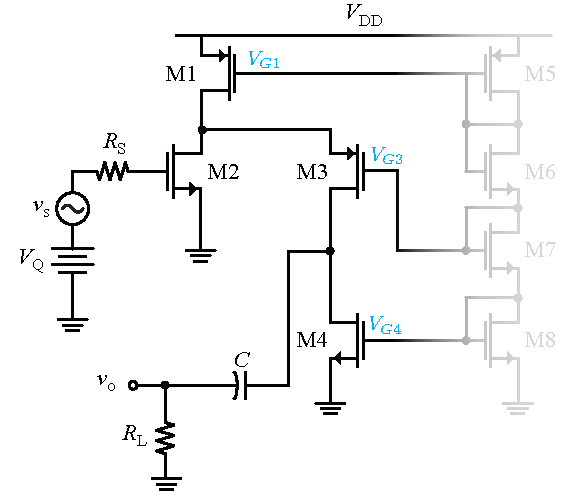
\includegraphics[scale=0.85]{17cascode_folded_declutter}
\caption{Schematic of an amplifier highlighting the signal path and ignoring biasing elements.}
\label{fig:17cascode_folded_declutter}
\end{figure}
%%%%%%%%%%%%%%%%%%%%%%%%%%%%%%%%%%%%%%%%%%%%
\newpage
%%%%%%%%%%%%%%%%%%%%%%%%%%%%%%%%%%%%%%%%%%%%
%                 FIGURE                   %
%%%%%%%%%%%%%%%%%%%%%%%%%%%%%%%%%%%%%%%%%%%%
\begin{figure}[t]
\centering
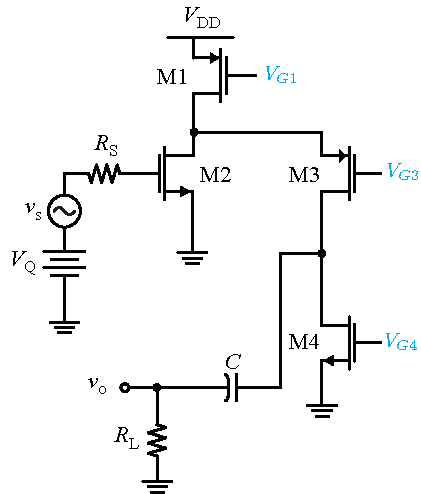
\includegraphics[scale=1]{18cascode_folded_dc}
\caption{Further simplification of the amplifier by noting that many transistors are biased with a nearly constant DC voltage.}
\label{fig:18cascode_folded_dc}
\end{figure}
%%%%%%%%%%%%%%%%%%%%%%%%%%%%%%%%%%%%%%%%%%%%
%                 FIGURE                   %
%%%%%%%%%%%%%%%%%%%%%%%%%%%%%%%%%%%%%%%%%%%%
\begin{figure}[H]
\centering
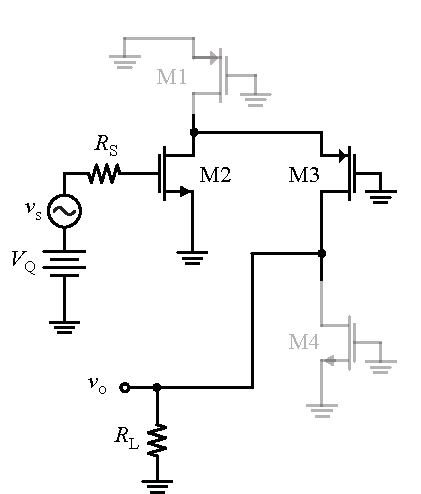
\includegraphics[scale=1]{19cascode_folded_ac}
\caption{AC schematic of the core amplifier consists of transistors M2/M3, known as a "folded cascode" amplifier.}
\label{fig:19cascode_folded_ac}
\end{figure}
%%%%%%%%%%%%%%%%%%%%%%%%%%%%%%%%%%%%%%%%%%%%
%             SUBSECTION 15.7.2            %
%%%%%%%%%%%%%%%%%%%%%%%%%%%%%%%%%%%%%%%%%%%%
\subsection{Eliminate More Clutter}
In the schematic of \emph{Fig.~\ref{fig:17cascode_folded_declutter}}, notice that $M1$ and $M4$ are biased with constant gate-source voltage, and only play an indirect role as far as the signal is concerned.  In fact, we can model them as current sources and simplify the schematic further, shown in \emph{Fig.~\ref{fig:18cascode_folded_dc}}.

Since $M1$ and $M4$ are providing DC currents, as far as the AC circuit is concerned they are open-circuits, as shown in \emph{Fig.~\ref{fig:19cascode_folded_ac}}.  With all these simplifications, we finally can see the essence of the circuit. It is simply an $NMOS$ common source stage followed by a $PMOS$ common gate stage.  This is similar to a cascode, except that it is "folded down", and aptly named the \textbf{"folded cascode"}\index{Amplifier!multi-stage!folded cascode}.  $M1$ provides the required DC bias for both $M2$ and $M3$.  Since $M4$ establishes the current in $M3$, the difference between the current of $M1$ and $M4$ flows into $M2$.

Why is the cascode folded?  Compared with a regular cascode, the second stage moves the DC bias voltage down, which may be required to drive another stage.  Furthermore, by folding the cascode, the voltage headroom\index{Amplifier!headroom} requirements are reduced.

Now let's put the circuit under the microscope to see if we missed anything.  Notice that in \emph{Fig.~\ref{fig:16cascode_folded}}, there is actually a current divider that we neglected.  The AC current generated by $M2$ is divided between $M3$, $M2$ ($r_o$), and $M1$.  We tacitly assumed that $M3$ has a much higher input conductance (approximately $g_m$) compared to the output conductance of $M1$, which is $\frac{1}{r_{o1}}$, and so we pretty much neglected the AC current flowing into $M1$.  Similarly, we lose a small amount of current into the output resistance of $M2$, which we ignored.  The only time we need to be careful about this approximation is when the load $R_L$ becomes very large, invalidating our assumption that the input impedance of $M3$ is $\frac{1}{g_m}$.  Also, if you were wondering, since $M1$ is not diode connected, its current is not mirrored to $M5$, even though they have the same $v_{gs}$.  Taking this all into consideration, the gain of the amplifier is given by:
    \begin{align}
        A_v &= -g_{m,2}\left(\frac{g_{m,3}}{g_{m,3} + \frac{1}{r_{o,1}} + \frac{1}{r_{o,2}}}\right)
                    \cdot \Big(R_L \parallel r_{o,4} \parallel \big((1 + g_{m,3} r_{o,1} \parallel r_{o,2})\big)\;r_{o,3}\\[0.5cm]
        \Aboxed{&\approx -g_{m,2}\,R_L}
        \text{\qquad\qquad\qquad\qquad}\textit{Folded cascode amplifier gain}
        \label{eq:folded_cascode_gain}
    \end{align} 
If the above equation is "obvious" to you, congratulations.  You have made it, and can now analyze multi-stage amplifiers by "inspection".  If not, don't worry, it just takes some time and practice.
%%%%%%%%%%%%%%%%%%%%%%%%%%%%%%%%%%%%%%%%%%%%
% \newpage
% %%%%%%%%%%%%%%%%%%%%%%%%%%%%%%%%%%%%%%%%%%%%%%%%%%%%%%%%%%%%%%%%%%%%%%%%%%%%%%%%%%%%%%%%
% %%%%%%%%%%%%%%%%%%%%%%%%%%%%%%%%%%%%%%%%%%%%%%%%%%%%%%%%%%%%%%%%%%%%%%%%%%%%%%%%%%%%%%%%
% %                                 SECTION 15.8                                         %
% %%%%%%%%%%%%%%%%%%%%%%%%%%%%%%%%%%%%%%%%%%%%%%%%%%%%%%%%%%%%%%%%%%%%%%%%%%%%%%%%%%%%%%%%
% %%%%%%%%%%%%%%%%%%%%%%%%%%%%%%%%%%%%%%%%%%%%%%%%%%%%%%%%%%%%%%%%%%%%%%%%%%%%%%%%%%%%%%%%
% \section{Chapter Summary}
% In this chapter we ...


%%%%%%%%%%%%%%%%%%%%%%%%%%%%%%%%%%%%%%%%%
%
%\subsection{External Loads}
%
%
%\begin{figure}
%\centering
%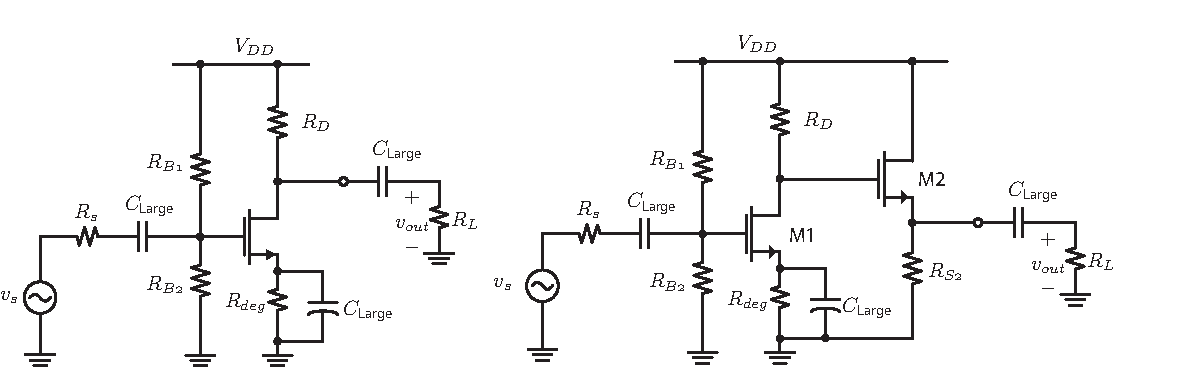
\includegraphics[scale=1]{22cs_cd_small_load}
%\caption{blank} \label{fig:blank}
%\end{figure}
%
% Many applications must drive external loads that are very low impedance compared to on-chip levels.
% These stages must drive high voltages/currents so linearity is a concern. We must consider “large signal” swing and distortion behavior (EE142).
% 
%
%
%%%%%%%%%%%%%%%%%%%%%%%%%%%%%%%%%%%%%%%%%
%
%\subsection{Source Follower for External Loads}
%
%
% Example: Speaker at 8 ohms versus Megaohms on-chip …
% In the example above, if $R_L$ is $8\Omega$, to get any gain we require very high current levels:
%
% 
%\begin{equation}
%	A_v \approx -g_m R_L = \frac{2 I_D}{V_{GS}-V_T} R_L
%\end{equation} 
%
% Say $V_{GS} - V_T = 0.2$V.  Then $I_D > 12.5$mA for unity gain.
% Follower is natural choice, but it can only “source” current (think in terms of large signals).
% For the case of the CD output stage, if we design set $I_{D2}$ of the follower to  12.5mA, then the output resistance $1/g_{m2}$ would give a gain of 0.5 for the output stage, but a \emph{much} larger gain can be realized on the CS stage, an overall win.
% 
%
%%%%%%%%%%%%%%%%%%%%%%%%%%%%%%%%%%%%%%%%%
%
%\subsection{Design Issue: DC Coupling}
%
%\begin{figure}
%\centering
%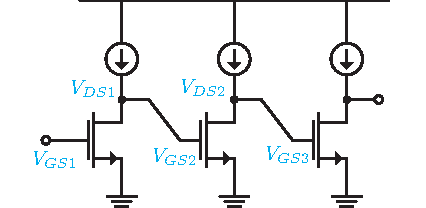
\includegraphics[scale=1]{23_cs_dc_levels}
%\caption{blank} \label{fig:blank}
%\end{figure}
%
% Output of one stage is directly connected to the input of the next stage, so we must consider DC levels … why? 
% Optimal $V_{DS}$ (say mid-rail) may not correspond with required $V_{GS}$ (for proper bias current). 
% Can solve the problem partially using level shifters and combinations of NMOS and PMOS.
% \textit{Constraint}: large inductors and capacitors are not available
% Is there a more robust way to do this without using inductors and capacitors ?  Yes !  We'll see that differential amplifiers have much more flexibility.
%
